%%%%%%%%%%%%%%%%%%%%%%%%%%%%%%%%%%%%%%%%%%%%%%%%%%%%%%%%%%%%%%%%%%%%%%%%%%
%%%%%                         CHAPITRE 1                            %%%%%%
%%%%%%%%%%%%%%%%%%%%%%%%%%%%%%%%%%%%%%%%%%%%%%%%%%%%%%%%%%%%%%%%%%%%%%%%%%

\lhead[\fancyplain{}{\leftmark}]%Pour les pages paires \bfseries
      {\fancyplain{}{}} %Pour les pages impaires
\chead[\fancyplain{}{}]%
      {\fancyplain{}{}}
\rhead[\fancyplain{}{}]%Pour les pages paires 
      {\fancyplain{}{\rightmark}}%Pour les pages impaires \bfseries
\lfoot[\fancyplain{}{}]%
      {\fancyplain{}{}}
\cfoot[\fancyplain{}{\thepage}]%\bfseries
      {\fancyplain{}{\thepage}} %\bfseries
\rfoot[\fancyplain{}{}]%
     {\fancyplain{}{\scriptsize}}


%%%%%%%%%%%%%%%%%%%%%%%%%%%%%%%%%%%%%%%%%%%%%%%%%%%%%%%%%%%%%%%%%%%%%%%%%%
%%%%%                      Start part here                          %%%%%%
%%%%%%%%%%%%%%%%%%%%%%%%%%%%%%%%%%%%%%%%%%%%%%%%%%%%%%%%%%%%%%%%%%%%%%%%%%

\chapter{State of the art}
\label{ch:1}

%======================================================	Résumé du chapitre

\begin{center}
\rule{0.7\linewidth}{.5pt}
\begin{minipage}{0.7\linewidth}
\smallskip

\textit{This chapter deals with the available prospects in motion capture (MoCap) in sports. It first present the standard marker-based (opto-electronic) systems for motion analysis and their limits. It briefly introduces some alternatives offered by Inertial Measurement Units (IMUs) or dept-field cameras. It then details the advent of markerless camera systems, which has been possible thanks to progress in machine learning. From 2D pose estimation to 3D joint angle determination, this is a new field which opens up new possiblities for motion analysis in a sports context. \newline \newline
This chapter is an up-to-date and slightly more detailed version of the introduction of the previously published paper "Pose2Sim: An End-to-End Workflow for 3D Markerless Sports Kinematics—Part 1: Robustness" \cite{Pagnon2021} }

%\smallskip
\end{minipage}
\smallskip
\rule{0.7\linewidth}{.5pt}
\end{center}

\minitoc
\newpage



\section{Overall context of kinematics in sports}

As coaching athletes implies observing and understanding their movements, motion capture (MoCap) is essential in sports. It helps improving movement efficiency, preventing injuries, or predicting performances. For the last few decades, marker-based systems have been considered the best choice for the analysis of human movement, when regarding the trade-off between ease of use and accuracy. However, these methods have proven to be much more challenging in a sports context than in a laboratory setting, and to be generally inappropriate \cite{Mündermann2006}.

\subsection{Marker-based systems}

Marker-based systems use a network of opto-electronic cameras. Each of these cameras are surrounded by a crown of infrared LEDs, which projects light toward the subject. The subject wears special markers, reflecting light back to the camera. The camera usually pre-processes the image to make it binary, and only outputs the coordinates of the detected marker candidates (Figure~\ref{fig_mk1}). 

If calibrated, using a network of these cameras allows for triangulating the 2D coordinates. Calibration involves knowing the cameras' intrinsic properties (such as focal length, optical center, distortion) as well as their extrinsic properties (their positions as regards to the global coordinate system.) See Chapter 2.2 on \nameref{sec:3D reconstruction} for more details. The reconstructed 3D marker positions are then used to optimize the posture of a physically consistent skeleton, scaled to each individual subject. In particular, this allows for obtaining 3D joint angles at each point in time.
% allows for 2 fois

\begin{figure}[hbtp]
	\centering
	\begin{subfigure}[b]{1\textwidth}
		\centering
		\def\svgwidth{\columnwidth}
		\fontsize{10pt}{10pt}\selectfont
		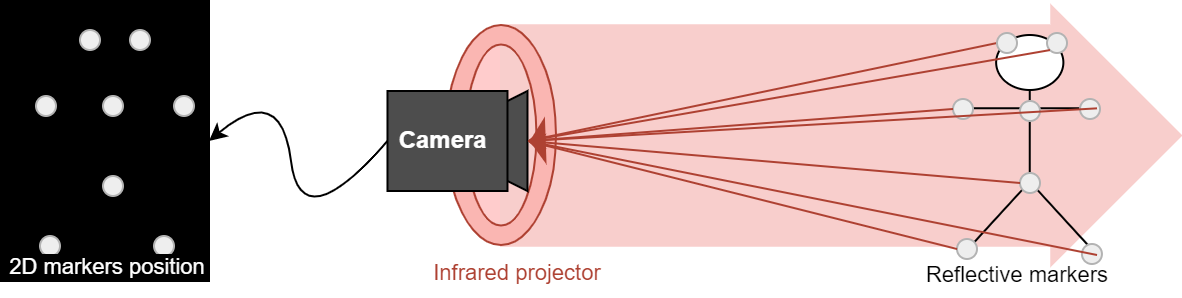
\includegraphics[width=\linewidth]{"../Chap1/Figure/marker_based_1.png"}
		\caption{An opto-electronic camera is traditionnaly surrounded by a crown of infrared LEDs, projecting light toward the subject. The subject wears markers, which reflect light back to the camera.}
		\label{fig_mk1}
	\end{subfigure}
	\qquad
	\begin{subfigure}[b]{1\textwidth}
		\centering
		\def\svgwidth{\columnwidth}
		\fontsize{10pt}{10pt}\selectfont
		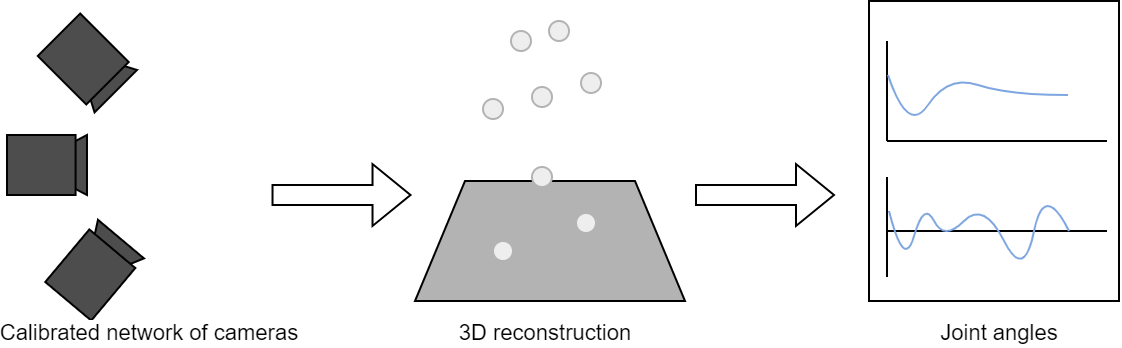
\includegraphics[width=\linewidth]{"../Chap1/Figure/marker_based_2.png"}
		\caption{Once calibrated, a network of these cameras allows for 3D reconstruction of marker positions. Marker coordinates are then used to infer the posture of the subject.}
		\label{fig_mk2}
	\end{subfigure}
	\caption{Principles of marker-based motion capture. (Figure~\ref{fig_mk1}) presents the functionning of an opto-electronic camera. (Figure~\ref{fig_mk2}) shows how a network of calibrated motion capture cameras helps obtaining joint angles.}
	\label{fig_mk}
\end{figure}

Indeed, reflective marker-based camera systems are complex to set up, are time-consuming, and are very expensive. They also require specific lightning conditions, and involve laying cables around. Moreover, markers may fall off the body due to sharp accelerations or sweat, as well as hinder the natural movement of athletes, which is likely to affect their warm-up and focus. While the accuracy of landmark location is claimed to be sub-millimetric in marker-based methods \cite{Topley2020}, marker placement is tedious, intrusive, prone to positioning variability from the operator \cite{Tsushima2003}, and subject to skin movement artifacts, especially on soft tissues. Della Croce et al. found out that inter-operator variations in marker placements range from 13 to 25 mm, which can propagate up to 10° in joint angle prediction \cite{Gorton2009,Croce1999}. For example, tissue artifacts account for up to a 2.5 cm marker displacement at the thigh, which can cause as much as a 3° error in knee joint angles tissues \cite{Benoit2015,Cappozzo1995}. Joint positions must be calculated explicitly in marker-based methods, which introduces more variability: these errors range up to 5 cm, which can contribute up to 3° of error in lower limb joint angles \cite{Leboeuf2019}. Nevertheless, since marker-based methods benefit from decades of research, they are still considered as the reference method for motion capture.

\subsection{IMU and RGBD systems}

How to use them (on limbs), accelerometer (linear acceleration), gyroscope (rotational speed), magnetometer (help define the constant while integrating other signals to get positions)

Consequently, other approaches based on alternative technologies have been investigated over the past years. For instance, wearable Inertial Measurement Units (IMUs) offer the advantage of getting away from all camera-related issues such as complex setup and calibration, limited field of view, self- and gear-occlusions, the need for a controlled environment, and they can operate in real-time \cite{Johnston2019,Chambers2015}. They still have the drawback of being an external equipment to still wear, involving high technical skills, and being sensitive to ferromagnetic disturbances. Above all, they are exposed to drift over time, and they are not suitable for joint positions assessment since these are obtained through multiple integrations of the original signal \cite{Ahmad2013}. 

Plutôt exactes, bien qu'une dernière étude \cite{Rekant2022} over 5° error for most motions.

Another approach involves depth-field cameras (RGBD), which give access to a 2.5D world (only the depth of the front facing plane of view is measured), or even to full 3D with a network of few RGBD cameras \cite{Carraro2017,Choppin2013,Colombel2020}. On the other hand, these cameras suffer from a sensitivity to lightning conditions, they work at lower framerates, and they are short-range \cite{Han2013}. 

\subsection{Markerless systems}

A recent breakthrough has come from Computer Vision. The explosion of deep-learning based methods from 2D camera videos, for which the research has skyrocketed around 2016 \cite{Wang2021a}, is related to the increase in storage capacities and huge improvements in GPU computing. A search on ScienceDirect for “deep learning 3D human pose estimation” produced fewer than 100 papers per year until 2015, and the number is now reaching almost 750 over the span of 5 years, fitting an exponential curve (Figure~\ref{fig_exp}).

It has rekindled interest from the Biomechanics community towards image-based motion analysis, which is where it all started with the invention of chronophotography in the 19th century by Marey in France, and Muybridge in the USA \cite{Baker2007}. Currently, two approaches coexist in human and animal motion analysis: on the one hand, computer vision using deep-learning techniques mostly focus on joint positions only; while the interest of biomechanics lies in kinematics, that involves joint angles. One of the main current challenges is to bridge the gap between these two worlds, and to take advantage of deep-learning technologies for kinematic analysis \cite{Cronin2021,Seethapathi2019}. 

\begin{figure}[hbtp]
	\centering
	\def\svgwidth{1\columnwidth}
	\fontsize{10pt}{10pt}\selectfont
	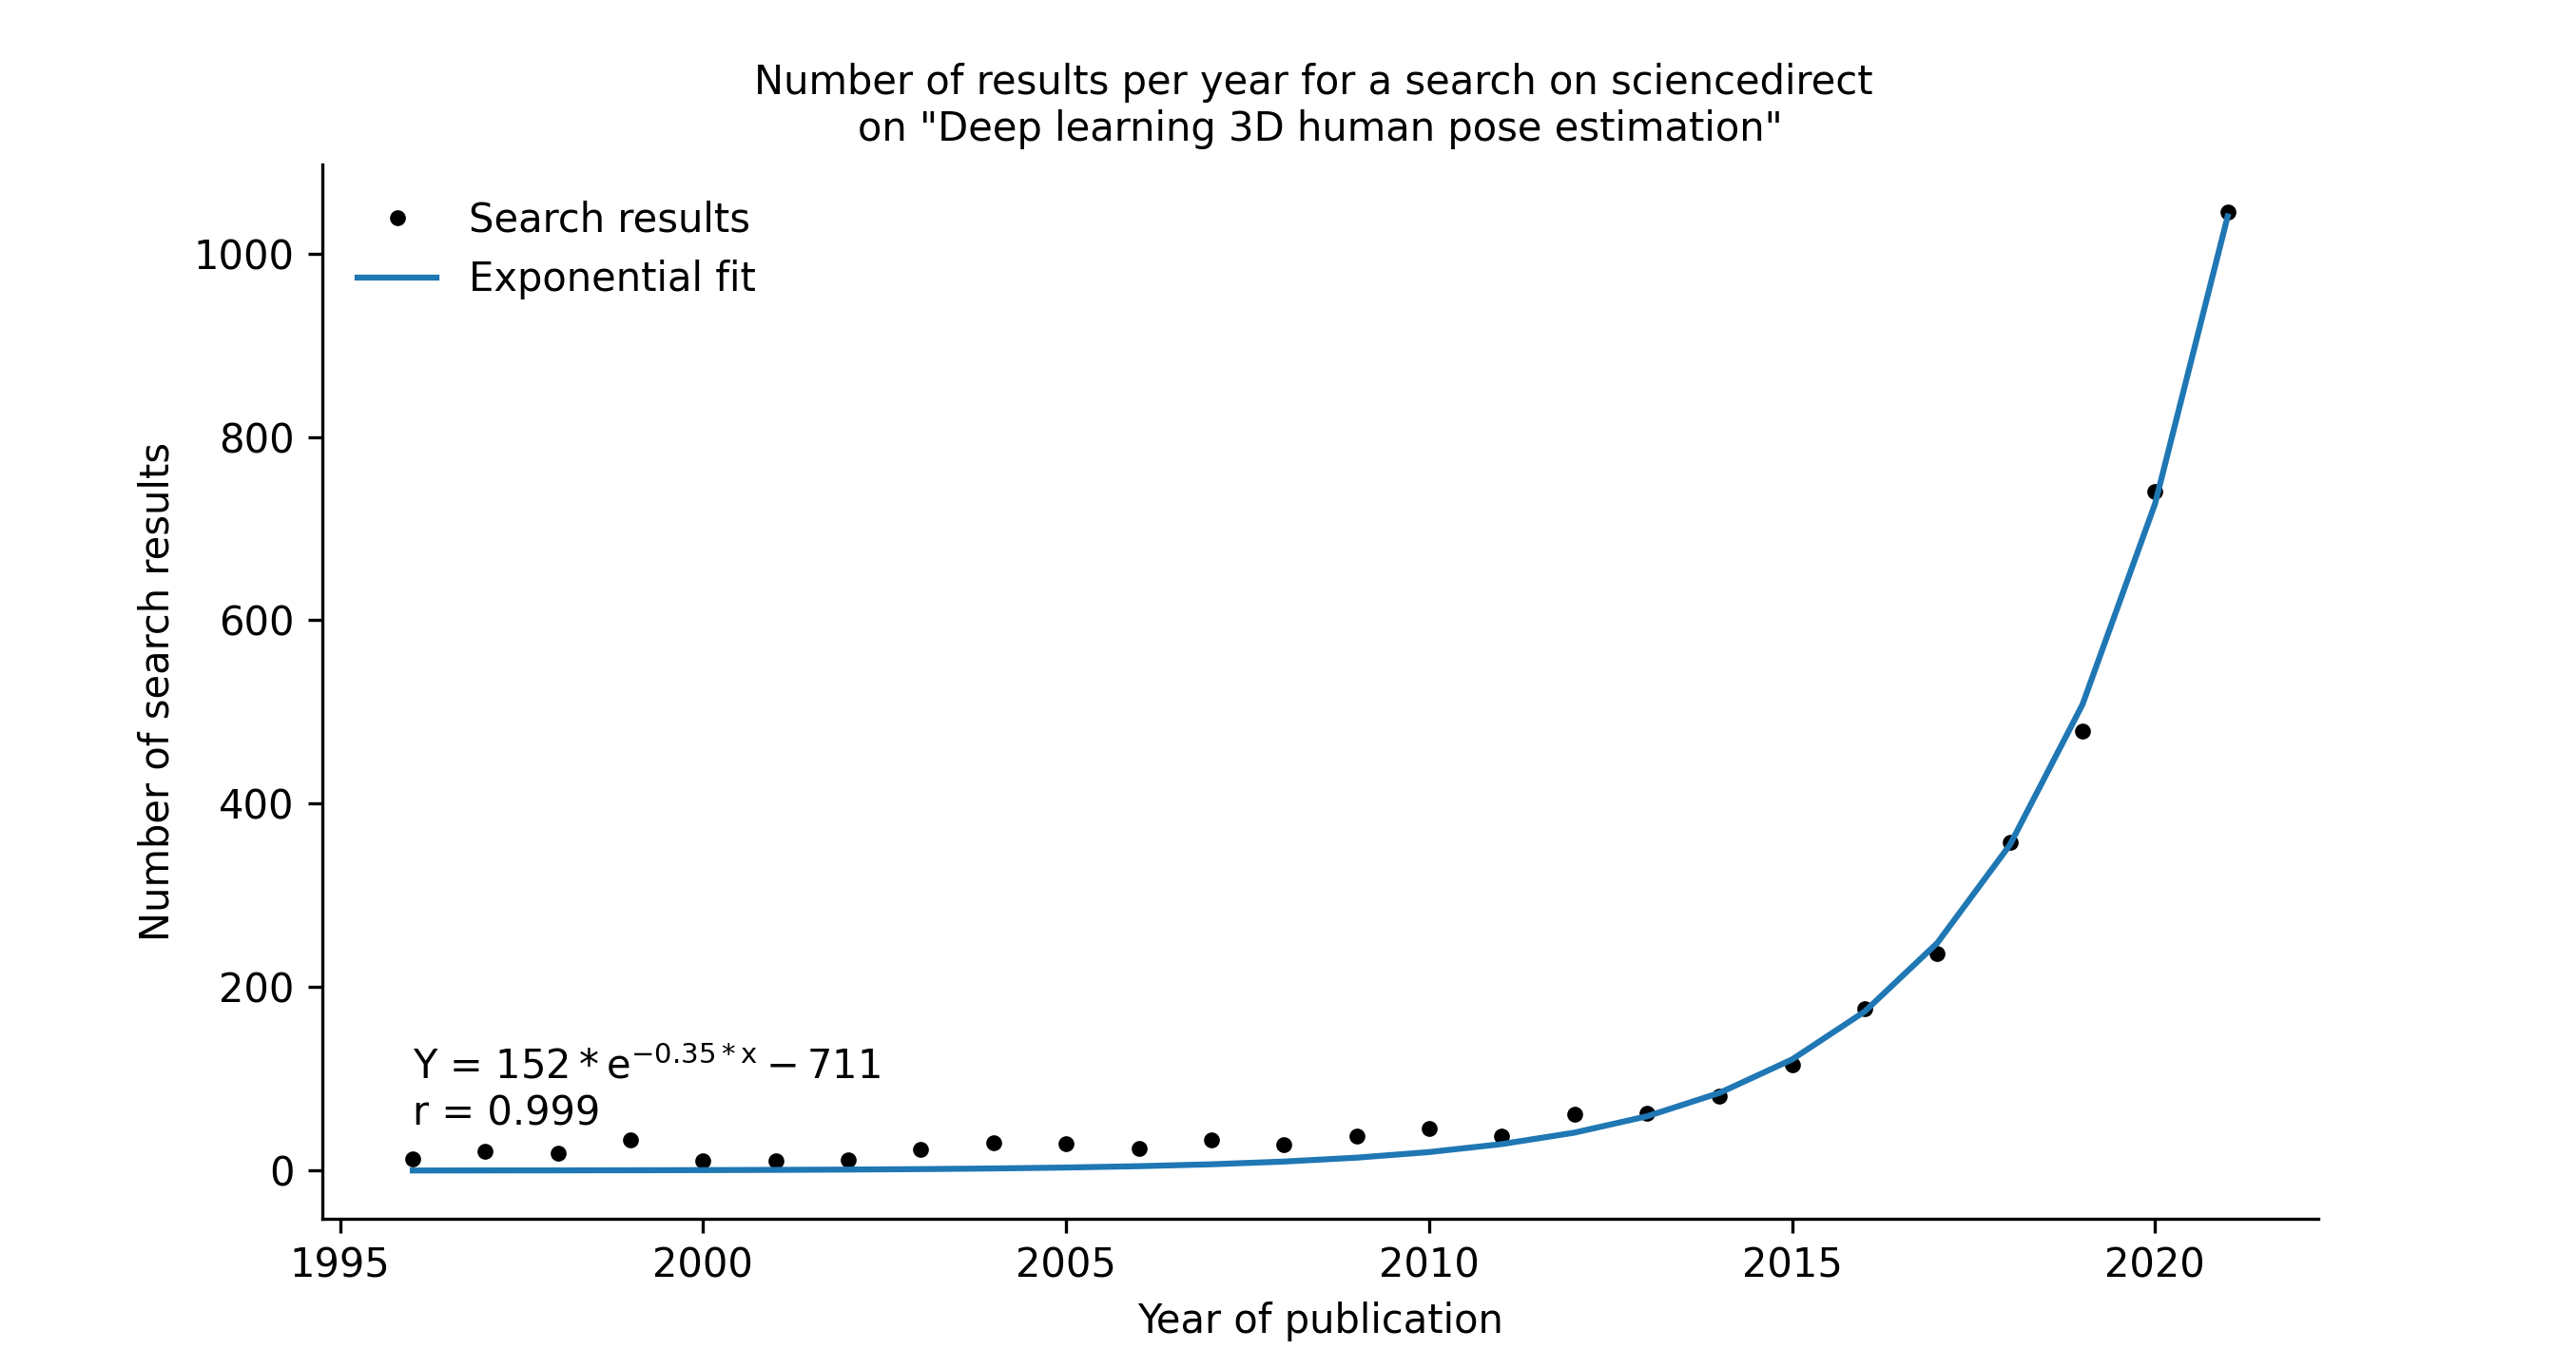
\includegraphics[width=\linewidth]{"../Chap1/Figure/Fig_exp.png"}
	\caption{The search for “deep learning 3D human pose estimation” (dots) fits an exponential curve (line). The search produced less than 100 results until 2015. Over the course of 5 years, the number has reached almost 750 of them, and is now well over a 1000 per year.}
	\label{fig_exp}
\end{figure}
\FloatBarrier

\section{2 dimensional analysis}

\subsection{2D pose estimation}

The most well-known off-the-shelf 2D human pose estimation solutions are OpenPose \cite{Cao2019}, and to a lesser extent AlphaPose \cite{Fang2017}. While both show similar results, OpenPose has the advantage of being a bottom-up approach, whose computation time does not increase with the number of persons detected \cite{Cao2019}. A bottom-up approach first detects all available joint keypoints, and then associates them to the right persons; while a top-bottom approach first detects bounding boxes around each person, and then finds joint keypoints inside of them. OpenPose has been trained on the CMU Panoptic Dataset \cite{Joo2015}, with 511 synchronized videos of multiple people in motion, alone or engaged in social activities. Another 2D pose estimation toolbox is DeepLabCut \cite{Mathis2018}, which was initially intended for markerless animal pose estimation, but which can be custom trained for the detection of any human or not human keypoint with a relatively small dataset. All of these tools are open-source. Other approaches have shown even better results on evaluation datasets (see review \cite{Chen2020}), but they are generally slower and not as widespread.
% attention, la citation de Chen concerne le monoculaire (ne pas supprimer, je la cite plus tard)

\subsection{2D kinematics from 2D pose estimation}

Some authors bridge 2D pose estimation to more biomechanically inspired goals, such as gait kinematics analysis. Kidzinski et al. present a toolbox for quantifying gait pathology that runs in a Google Colab \cite{Kidziński2020}. Stenum et al. evaluate gait kinematics calculated from OpenPose input concurrently with a marker-based method. Mean absolute error of hip, knee and ankle sagittal angles were 4.0°, 5.6° and 7.4° \cite{Stenum2021}. Liao et al. have not released their code, but they use OpenPose outputs to train a model invariant to view \cite{Liao2020}. Viswakumar et al. perform direct calculation of the knee angle from an average phone camera processed by OpenPose \cite{Viswakumar2019}. They show that OpenPose is robust to challenging clothing such as large Indian pants, as well as to extreme lightning conditions. Other sports activities have been investigated, such as lower body kinematics of vertical jump \cite{Drazan2021} or underwater running \cite{Cronin2019}. Both works train their own model with DeepLabCut. Serrancoli et al. fuse OpenPose and force sensors to retrieve joint dynamics in a pedaling task \cite{Serrancolí2020}. 


\section{3 dimensional analysis}

\subsection{3D pose estimation}

There are a lot of different approaches for markerless 3D human pose estimation and listing them all is beyond our scope (see review \cite{Wang2021a}]). Some more ancient ones are not based on deep-learning and require specific lightning and background conditions, such as visual-hull reconstruction \cite{Ceseracciu2014}. Some directly lift 3D from a single 2D camera (see review \cite{Chen2020}), with different purposes: one estimates the positions of a set of keypoints around the joint instead of determining only the joint center keypoint, so that axial rotation along the limb is solved \cite{Fisch2020}; SMPL and its sequels retrieve not only joint positions and orientations, but also body shape parameters \cite{Loper2015}; while XNect primarily focuses on real time \cite{Mehta2020}. A few approaches even strive to estimate 3D dynamics and contact forces from a 2D video input \cite{Rempe2021,Li2019}. Rempe et al. solve occlusions from a 2D input \cite{Rempe2020}, but this remains a probabilistic guess that may be unsuccessful in case of unconventional positions of hidden limbs, whereas using more cameras would have given more trustworthy results . Haralabidis et al. fuse OpenPose results from a single monocular video and two IMU outputs, and solve kinematics of the upper body in OpenSim (an open-source biomechanical 3D analysis software \cite{Delp2007,Seth2018}) in order to examine the effects of fatigue on boxing \cite{Haralabidis2020}.

Some research attempts to solve 3D pose estimation from a network of uncalibrated cameras, i.e., cameras whose extrinsic parameters (translation and rotation with respect to the coordinate system), intrinsic parameters (focal length, pixel size, etc.), and distortion coefficients are not known. It either uses 2D pose estimations of each view as visual cues to calibrate on \cite{Takahashi2018}, or an adversarial network that predicts views of other cameras, compares them to real views, and adjusts its calibration accordingly \cite{Ershadi-Nasab2021}. Dong et al. recover 3D human motion from unsynchronized and uncalibrated videos of a repeatable movement found on internet videos (such as a tennis serve performed by a celebrity) \cite{Dong2020}. Using uncalibrated videos is still a very experimental trend, that would require more research before being used in biomechanics.

We choose to focus on the methods that estimate 3D pose by triangulating 2D pose estimations from a network of multiple calibrated cameras. The classical evaluation metric is the MPJPE (Mean Per Joint Position Error), which is the average Euclidian distance between the estimated and the ground truth joint coordinate. Most methods take OpenPose as an input for triangulation, and more specifically the body\_25 model. Labuguen et al. evaluate 3D joint positions of a pop dancer with a simple Direct Linear Transform triangulation (DLT \cite{Hartley1997,Miller1980}) from 4 cameras \cite{Labuguen2020}. Apart from the upper body for which error goes up to almost 700 mm, the average joint position error is about 100 mm. Nakano et al. examine three motor tasks (walking, countermovement jumping, and ball throwing), captured with 5 cameras and triangulated with the same methods, with a subsequent Butterworth filter \cite{Nakano2019}. 47\% of the errors are under 20 mm, 80\% under 30 mm, and 10\% are above 40 mm. The largest errors are mostly caused by OpenPose wrongly tracking a joint, for example by swapping the left and the right limb, what causes large errors up to 700 mm. This may be fixed either by using a better 2D pose estimator, or by using more cameras to reduce the impact of an error on a camera, or else by considering the temporal continuity in movement. 

Slembrouck at al. go a step further and tackle the issue of limb swapping and of multiple persons detection \cite{Slembrouck2020}. In case of multiple persons detection, one needs to make sure they triangulate the person detected on one camera to the same person detected on the other ones. Slembrouck et al. manage to associate persons across cameras by examining all the available triangulations for the neck and mid-hip joints: the persons are the same when the distance between the triangulated point and the line defined by the detected point and the camera center is below a certain threshold. They only focus on lower limb. Their first trial features a person running while being filmed by seven cameras, whereas their second one involves a person doing stationary movements such as squats while filmed by 3 cameras. After filtering, the average positional error in the first case is about 40 mm, and it is roughly 30 mm in the second case (less than 20 mm for the ankle joint). Other authors deal with the multiperson issue in a slightly different way \cite{Bridgeman2019,Chu2021,Dong2019}. In average, if the detected persons are correctly associated and the limbs don’t swap, the average joint position error for an OpenPose triangulation is mostly below 40 mm.

Some triangulation methods not based on OpenPose reach even better results on benchmarks, although it comes at the cost of either requiring heavy computations, or of being out of reach for non-expert in computer vision. The classic approach is to detect probability maps for each joint, to assume that the maximum probability is the actual 2D joint position, and then to triangulating these scalar positions. Instead of this, the main two state-of-the art methods directly perform a volumetric triangulation of the heatmaps, and only then take the maximum probability. By working this way, they keep all the information available for as possible for as long as possible. They manage to lower their MPJPE to about 20 mm \cite{He2020,Iskakov2019}.


\subsection{3D kinematics from 3D pose estimation}

Instead of just working on 3D joint positions, the issue of 3D markerless kinematics (i.e., gait parameters and joint angles) is starting to be tackled. Zago et al. evaluate gait parameters computed by triangulating 2 videos processed by OpenPose, and notice that straight gait direction, longer distance from subject to camera, and higher resolution make a big difference in accuracy \cite{Zago2020}. D’Antonio at al. perform a simple triangulation of the OpenPose output of two cameras, and compute direct Euler angle calculations for the lower limb \cite{D'Antonio2021}. They compare their results to IMU and point out that errors are higher for running than for walking, and are also rather inconsistent: up to 14°, although they can get down to 2 to 7° if the two cameras are set laterally rather than in the back of the subject. Theia3D, a recent commercial (and not open) solution, estimates the positions of a set of keypoints around the joint, and then uses a multi-body optimization approach to solve inverse kinematics \cite{Kanko2021a,Kanko2021b}. They notice an offset in hip and ankle angles between their markerless system and the reference marker-based one, likely doe to different skeletal models. Once this offset is removed the root mean square error (RMSE) in lower limb roughly ranges between 2 and 8° for flexion/extension and abduction/adduction angles, and up to 11.6° for internal/external rotation. AniPose broadens the perspective to the kinematics of any human or animal with a DeepLabCut input, instead of OpenPose. They offer custom temporal filters, as well as spatial constraints on limb lengths \cite{Karashchuk2021}.


\section{Statement of need}

According to Atha \cite{Atha1984}, an ideal motion analysis system involves the collection of accurate information, the elimination of interference with natural movement, and the minimization of capture and analysis times. Yet, despite a marker-based system gives relatively accurate results, it requires placing markers on the body, which can hinder natural movement, and which are not it is hard to set up outdoors or in context, and it is strenuous to analyse. 

Coaches usually investigate performance indicators and compare athletes, and compare with subjective visual observation 
However, despite these benefits, investing in technology has its pitfalls: the information gathered can be unhelpful, or inaccurate, or not easily interpretable, or not implementable in the context of sports \cite{Windt2020}. 

The emergence of markerless kinematics opens up new possibilities. Indeed, the interest in deep-learning pose estimation neural networks has been growing fast since 2015 \cite{Zheng2022}, which makes it now possible to collect accurate and reliable kinematic data without the use of physical markers. OpenPose, for example, is a widespread open-source software which provides 2D joint coordinate estimations from videos. These coordinates can then be triangulated in order to produce 3D positions. Yet, when it comes to the biomechanical analysis of human motion, it is often more useful to obtain joint angles than their XYZ positions in space. Joint angles allow for better comparison among trials and individuals, and they represent the first step for other analysis such as inverse dynamics.

OpenSim is another widespread open-source software which helps compute 3D joint angles, usually from marker coordinates. It lets scientists define a detailed musculoskeletal model, scale it to individual subjects, and perform inverse kinematics with customizable biomechanical constraints. It provides other features such as net calculation of joint moments or individual muscle forces resolution, although this is out of the scope of our contribution.

The goal of Pose2Sim is to build a bridge between the communities of computer vision and biomechanics, by providing a simple and open-source pipeline connecting the two aforementioned state-of-the-art tools: OpenPose and OpenSim. Pose2Sim has already been used and tested in a number of situations (walking, running, cycling, balancing, swimming, boxing), and published in peer-reviewed scientific publications \cite{Pagnon2021,Pagnon2022} assessing its robustness and accuracy. The combination of its ease of use, customizable characteristics, and high robustness and accuracy makes it promising, especially for "in-the-wild" sports movement analysis.

So far, little work has been done towards obtaining 3D angles from multiple views \cite{Zheng2022}. However, two software applications are worth mentioning. Anipose \cite{Karashchuk2021} proposes a Python open-source framework which allows for joint angle estimation with spatio-temporal constraints, but it is primarily designed for animal motion analysis. Theia3D \cite{Kanko2021a} is a software application for human gait kinematics from videos. Although the GUI is more user friendly, it is not open-source nor easily customizable. Our results on inverse kinematics were deemed good when compared to marker-based ones. See \cite{Pagnon2022} for more details on concurrent accuracy with other systems.

---

Currently, reference methods in sports analysis remain marker-based. These methods, also known as MoCap (motion capture) procedures, are mostly concerned with accuracy, despite the fact that marker placement hinders natural movement and is time consuming. Therefore, several markerless technologies are being examined to solve these issues. The main candidates are either based on Inertial Measurement Units (IMUs) [2,3], depth cameras [4,5,6], or a network of RGB cameras [7,8,9]. IMUs avoid all camera-related issues such as complex setup and calibration, potential self- and gear obstructions, and can operate in real time; however, they need to be worn by the athlete and are sensitive to drift over time, and to ferromagnetic disturbances. Depth cameras offer more information than RGB cameras but they hardly work in direct sunlight nor at a distance over 5 m [10]. On the other hand, a network of RGB cameras does not assume any particular environment, and it does not hinder the athlete’s movement and focus, but it requires delicate calibration, complex setup, large storage space, and high computational capacities. The technology, however, is still maturing and some light-weight systems such as BlazePose [11] or UULPN [12] are being proposed, which can operate in real time on a mobile phone; however, they are still not quite as accurate as required for quantitative motion analysis.

We focus on the latter approach, and more specifically on methods triangulating 2D joint center estimations from a network of several calibrated RGB cameras. The most common evaluation metric is the Mean Per Joint Position Error (MPJPE), which is the average Euclidian distance between the estimated joint coordinate and its ground truth. A large part of studies investigating 3D joint center estimation choose to triangulate the output of OpenPose [13], a deep-learning algorithm estimating 2D joint coordinates from videos. Their MPJPE usually lies between 30 and 40 mm [14,15,16]. Ankle MPJPEs are within the margin of error of marker-based technologies (1–15 mm), whereas knee and hip MPJPEs are greater (30–50 mm). These errors are systematic and likely due to “ground-truth” images being mislabeled in the training dataset [17]. Triangulation from other 2D deep-learning algorithms (such as AlphaPose [18] and DeepLabCut [19]) have also been compared [17]. AlphaPose results are similar to OpenPose’s; however, DeepLabCut errors are substantially higher.

Numerous studies have focused on the accuracy of 3D joint center estimation, but far fewer have examined 3D joint angle estimation. D’Antonio et al. computed direct flexion-extension angles for the lower limb from two cameras processed with OpenPose [20]. Range of Motion (ROM) errors lay between 2.8° and 14.1°. Wade et al. calculated frontal and sagittal knee and hip angles with OpenPose, AlphaPose, and DeepLabCut [21]. They deemed the method accurate enough for assessing step length and velocity, but not for joint angle analysis. AniPose offers a toolkit for triangulating 2D poses from DeepLabCut [22]. To our knowledge, it has only been concurrently validated for index finger angles in the sagittal plane, resulting in a root-mean-square error of 7.5 degrees [23]. Theia, a commercially available software package for markerless analysis, uses its own patent-protected 2D pose estimator and triangulation procedure, and runs a skeletal model to constrain the results to physically consistent poses and movements [24]. Their root-mean-square error (RMSE) compared to a marker-based method ranged between 2.6° and 13.2°.


\section{Exemples}

\FloatBarrier
\subsection{Figures}

La Figure~\ref{figure_multiple} est un exemple d'intégration d'une figure multiple. \\
Il est bien entendu possible de faire référence à la Figure~\ref{figure_subplot} ou à la Figure~\ref{figure_polaire}.

\begin{figure}[hbtp]
	\centering
	\begin{subfigure}[b]{0.8\textwidth}
		\centering
		\def\svgwidth{\columnwidth}
		\fontsize{10pt}{10pt}\selectfont\input{../Chap1/Figure/Figure_2.pdf_tex}
		\caption{Exemple subplot} 
		\label{figure_subplot}
	\end{subfigure}
	\qquad
	\begin{subfigure}[b]{0.7\textwidth}
		\centering
		\def\svgwidth{\columnwidth}
		\fontsize{10pt}{10pt}\selectfont\input{../Chap1/Figure/Figure_3.pdf_tex}
		\caption{Exemple diagramme polaire} 
		\label{figure_polaire}
	\end{subfigure}
	\caption{Exemple de Figures multiple} 
	\label{figure_multiple}
\end{figure}



\FloatBarrier
\subsection{Tableaux}

Générateur en ligne \href{http://www.tablesgenerator.com/latex_tables}{ici}. \\

Un exemple de tableau générée par cet outil est présenté Table~\ref{tableau_exemple}.

\begin{table}[]
\centering
\begin{tabular}{c|c|c|c|}
\cline{2-4}
                               & \textbf{A}                 & \textbf{B} & \textbf{C} \\ \hline
\multicolumn{1}{|c|}{$\alpha$} & \multicolumn{3}{c|}{\textit{fusion}}                 \\ \hline
\multicolumn{1}{|c|}{$\beta$}  & \multirow{2}{*}{\textit{}} & \textit{1} & \textit{2} \\ \cline{1-1} \cline{3-4} 
\multicolumn{1}{|c|}{$\Delta$} &                            & \textit{3} & \textit{4} \\ \hline
\end{tabular}
\caption{Exemple de tableau}
\label{tableau_exemple}
\end{table}
